\documentclass[a4paper,12pt]{article}
	\usepackage{graphicx}
	\usepackage[utf8]{inputenc}
	\usepackage[T1]{fontenc}
	\usepackage{listings}
	\usepackage{color}
	\usepackage{amsmath}

	\definecolor{dkgreen}{rgb}{0,0.6,0}
	\definecolor{gray}{rgb}{0.5,0.5,0.5}
	\definecolor{mauve}{rgb}{0.58,0,0.82}

	\lstset{frame=tb,
	  language=Python,
	  aboveskip=3mm,
	  belowskip=3mm,
	  showstringspaces=false,
	  columns=flexible,
	  basicstyle={\small\ttfamily},
	  numbers=none,
	  numberstyle=\tiny\color{gray},
	  keywordstyle=\color{blue},
	  commentstyle=\color{dkgreen},
	  stringstyle=\color{mauve},
	  breaklines=true,
	  breakatwhitespace=true
	  tabsize=3
	}
	\title{ Mecânica Clássica I}
	\author{\small André Del Bianco Giuffrida\\ \small IFSC - USP\\ \small andre.giuffrida@usp.br}
	\date{}
\begin{document}
\maketitle
	Para uma particula com massa m na presença de um potêncial V(x) dado por:
	
		
		\[ V(x)= ax^2 -bx^3\]
		
		\begin{figure}[h]
			\centering
			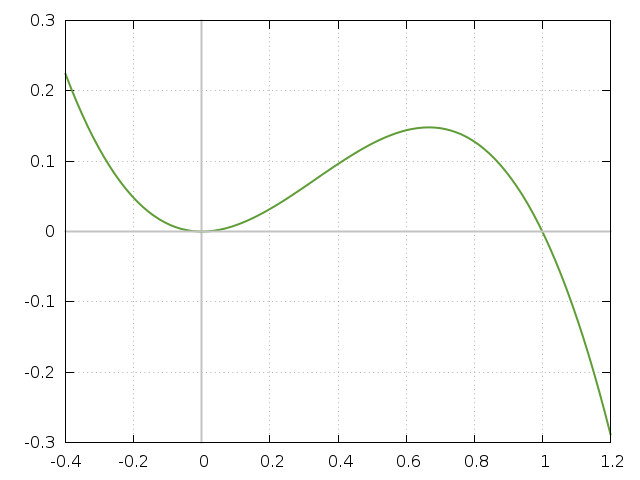
\includegraphics[scale=0.6]{5o0.png}
			\caption{$V(x)$}
		\end{figure}

	Note que na região próxima a origem temos um vale de potencial, o que significa que se a energia inicial não for suficientemente grande para fezer com que x ultapasse o maximo de potencial, a particula estará confinada na região próxima a origem (como um oscilador).
	Devemos então calcular os pontos de máximo e mínimo para o potencial:
	
	\[ \frac{dV(x)}{dx} = 2ax -3bx^2 \]
	e igualando a zero temos:
	\[ 2a = 3bx  \to x=\frac{2a}{3b}  \]
	ou seja o potencial tem um máximo local em $\frac{2a}{3b}$ e podemos notar que calculamos $-F(x)$ pois:
	
	\begin{figure}[h]
			\centering
			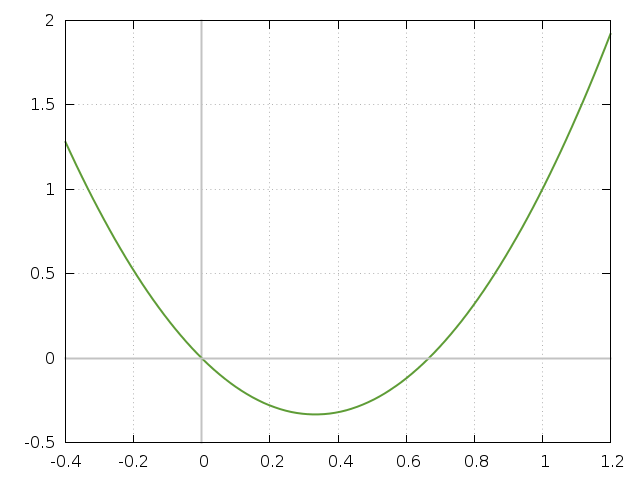
\includegraphics[scale=0.6]{5o1.png}
			\caption{$F(x)$}
		\end{figure}
	
	\[ F(x) = -\frac{dV(x)}{dx}\]
	ou seja:
	\[ F(x) = -2ax + 3bx^2 \]
	
		Note que a força é sempre oposta a x no intervalo $x < \frac{2a}{3b}$ ou seja ela se comporta como uma força restauradora nesse intervalo.
		Porém, se a partícula conseguir atingir um valor de $x$ tal que a força acomanha o movimento ( $x > \frac{2a}{3b}$ ) o movimento se torna um acelerado ($\propto x^2$) quanto mais longe da origem a particula estiver maior vai ser a força dela.
		Note que para valores negativos de $x$ a partícula estará sob a atuação de uma força $>0$ oposta a seu movimento, ou seja perdendo energia cinética e ganhando potencial como era esperado.\\
		
		\indent Para fazer-mos uma análise mais profunda teremos que calcular a energia total do sistema:
		\[ E = T + V \] Onde $T$ é a energia cinética do sistema.\\ \\
		Pelas condições iniciais temos:
		\[ V(0) = 0 \quad \text{implica que:} \quad E = \frac{mv_{0}^{2}}{2}\]
		
		Como o potêncial máximo para que a particula fique aprisionada em volta da origem é: \[ V\Big(\frac{2a}{3b}\Big) = a\Big(\frac{2a}{3b}\Big)^2 -b\Big(\frac{2a}{3b}\Big)^3 \]
		\[ V\Big(\frac{2a}{3b}\Big) \quad = \quad \frac{4a^3}{9b^2} - \frac{8a^3}{27b^2} \quad = \quad \frac{4a^3}{9b^2}(1-\frac{2}{3}) \quad = \quad \frac{4a^3}{27b^3}\]
		E por conservação de energia \[ E_f - E_i = 0\] Oonde $E_i$ e $E_f$ são respectivamente a energia final e inicial do sistema.
		Sendo assim:
		\[ (T_f + V_f) - (T_i + V_i) = 0\]
		Como $ V_i = 0 = T_f$
		\[V_f = T_i\]
		Temos que $T_i = T(0)$ e $V_f = V(\frac{2a}{3b})$ obtemos a relação:
		
		\[ \frac{mv_{c}^{2}}{2} = \frac{4a^3}{27b^3} \]
		Sendo assim,
		\[ v_c = \sqrt{\frac{8a^3}{27b^3 m}} \]
	\end{document}
	
